\documentclass[14pt, a4paper]{extarticle}
\usepackage[T2A]{fontenc}
\usepackage[utf8]{inputenc}
\usepackage[english, russian]{babel}
\usepackage[left=30mm, right=10mm, top=20mm, bottom=20mm]{geometry}

\usepackage{float}

\usepackage{misccorr}
\usepackage{indentfirst}
\usepackage{graphicx}
\usepackage{setspace}
\onehalfspacing

% Настройка переносов
\usepackage{hyphenat}
\hyphenpenalty=50
\tolerance=1000

% Отступ первой строки (красная строка)
\setlength{\parindent}{1.25cm}

% Заголовки section по центру, жирный шрифт
\makeatletter
\renewcommand\section{\@startsection {section}{1}{\z@}%
                                   {-3.5ex \@plus -1ex \@minus -.2ex}%
                                   {2.3ex \@plus.2ex}%
                                   {\centering\normalfont\Large\bfseries}}
\makeatother

% Заголовки subsection по центру, жирный шрифт
\makeatletter
\renewcommand\subsection{\@startsection {subsection}{2}{\z@}%
                                   {-2.5ex \@plus -1ex \@minus -.2ex}%
                                   {1.5ex \@plus.2ex}%
                                   {\centering\normalfont\large\bfseries}}
\makeatother

% Нумерация подподпунктов отключена
\setcounter{secnumdepth}{2}
\setcounter{tocdepth}{2}

% Точки в списке литературы
\makeatletter
\renewcommand\@biblabel[1]{#1.}
\makeatother

\begin{document}

% ===================== ТИТУЛЬНЫЙ ЛИСТ =====================

\thispagestyle{empty}
\nopagebreak

\noindent
\begin{minipage}[c]{0.2\textwidth}
    
\includegraphics[width=0.8\linewidth]{tim-logo.png}
\end{minipage}%
\hfill
\begin{minipage}[c]{0.8\textwidth}
    {\scriptsize
    \begin{center}
        \textbf{МИНИСТЕРСТВО СЕЛЬСКОГО ХОЗЯЙСТВА РОССИЙСКОЙ ФЕДЕРАЦИИ}
        
        ФЕДЕРАЛЬНОЕ ГОСУДАРСТВЕННОЕ БЮДЖЕТНОЕ ОБРАЗОВАТЕЛЬНОЕ УЧРЕЖДЕНИЕ ВЫСШЕГО ОБРАЗОВАНИЯ
        
        \textbf{«РОССИЙСКИЙ ГОСУДАРСТВЕННЫЙ АГРАРНЫЙ УНИВЕРСИТЕТ -- МСХА имени К.\,А.~ТИМИРЯЗЕВА»}
        
        \textbf{(ФГБОУ ВО РГАУ -- МСХА имени К.\,А.~Тимирязева)}
    \end{center}
    }
\end{minipage}

\bigskip
\noindent\rule{\textwidth}{0.4pt}\\[-2.0ex]
\rule{\textwidth}{0.4pt}

{\small
\begin{center}
Институт экономики и управления

Кафедра статистики и кибернетики

Направление: 09.03.02 Информационные системы и технологии

Направленность: Большие данные и машинное обучение

Методы и средства проектирования информационных систем и технологий
\end{center}
}

\vspace{-0.3cm}

{\Large
\begin{center}
\textbf{КУРСОВОЙ ПРОЕКТ}
\end{center}
}

\vspace{-0.3cm}

\begin{center}
    \small на тему: «Проектирование и разработка веб-приложения «Цифровой агроном» с ИИ-ассистентом для поддержки принятия решений в растениеводстве».
\end{center}

\vspace{0.3cm}

\begin{flushright}
    \small
    \begin{tabular}{l}
        Выполнил:\\
        Студент 3 курса группы Д-Э-311\\
        Бондарев И.\,А.\\[0.5ex]
        Дата регистрации КП\\
        на кафедре: \rule{4cm}{0.4pt}\\[0.15cm]
        Допущен к защите\\[0.1cm]
        Руководитель:\\[0.1cm]
        \rule{6cm}{0.4pt}\\
        \hspace*{0.5cm}{\footnotesize учёная степень, учёное звание, ФИО}\\[0.25cm]
        Члены комиссии:\\[0.1cm]
        \rule{6cm}{0.4pt}\hfill\rule{2cm}{0.4pt}\\
        {\footnotesize учёная степень, учёное звание, ФИО}\hfill{\footnotesize подпись}\\[0.1cm]
        \rule{6cm}{0.4pt}\hfill\rule{2cm}{0.4pt}\\
        {\footnotesize учёная степень, учёное звание, ФИО}\hfill{\footnotesize подпись}\\[0.1cm]
        \rule{6cm}{0.4pt}\hfill\rule{2cm}{0.4pt}\\
        {\footnotesize учёная степень, учёное звание, ФИО}\hfill{\footnotesize подпись}\\[0.25cm]
        Оценка \rule{6cm}{0.4pt}\\[0.15cm]
        Дата защиты \rule{5cm}{0.4pt}
    \end{tabular}
\end{flushright}

\vspace{0.3cm}
\begin{center}
    Москва 2026
\end{center}

% ===================== СОДЕРЖАНИЕ =====================

\newpage
\tableofcontents

% ===================== ВВЕДЕНИЕ =====================

\newpage
\addcontentsline{toc}{section}{Введение}
\section*{Введение}

    В современной цифровой среде актуальность интеллектуальных систем поддержки принятия решений в сельском хозяйстве существенно возрастает. Растениеводство сталкивается с рядом вызовов: изменение климата, распространение новых болезней, необходимость оптимизации ресурсов. Традиционные методы консультации не всегда доступны фермерам в удалённых регионах.

    Цифровая трансформация сельского хозяйства (AgriTech) предлагает решения на базе искусственного интеллекта. Зарубежные продукты (Plantix, Climate FieldView) \cite{plantix}\cite{climate} демонстрируют возможность автоматической диагностики болезней и прогнозирования урожайности. Однако многие из них недоступны в РФ, требуют платной подписки или не учитывают российскую специфику.

    В условиях санкционного давления возникли проблемы с доступом к зарубежной инфраструктуре разработки (PyPI.org, GitHub, Hugging Face) \cite{blocks}, что потребовало поиска альтернативных путей: использование зеркал, ручную установку совместимых версий, отказ от проблемных библиотек.

    Целью данной работы является проектирование, разработка и экспериментальная апробация веб-приложения «Цифровой агроном» с ИИ-ассистентом, обеспечивающего прогнозирование урожайности на основе ML-модели и консультационную поддержку.

    Для достижения цели требуется решить следующие задачи:
    \begin{enumerate}
        \item Провести анализ систем поддержки принятия решений в сельском хозяйстве.
        \item Изучить проблемы импортозамещения и доступности технологий в РФ.
        \item Выбрать оптимальный стек технологий.
        \item Спроектировать модульную архитектуру веб-приложения.
        \item Реализовать программный прототип.
        \item Провести тестирование и оценить качество работы системы.
    \end{enumerate}

    Объектом исследования являются процессы поддержки принятия решений в растениеводстве. Предметом исследования выступают методы машинного обучения для прогнозирования урожайности и технологии построения ИИ-ассистентов.

    Практическая значимость работы заключается в возможности использования разработанного приложения для помощи фермерским хозяйствам.

    Структура работы включает введение, две главы (теоретическую и практическую), заключение, библиографический список и приложение.

% ===================== ГЛАВА 1 =====================

\newpage
\section{Глава 1. Теоретическая часть}

\subsection{Эволюция и современное состояние систем поддержки принятия решений в сельском хозяйстве}

    История развития систем поддержки принятия решений (СППР) в сельском хозяйстве отражает общую эволюцию информационных технологий — от простых статистических отчётов до сложных интеллектуальных систем \cite{evolution}.

    На начальном этапе (1960–1980-е годы) использовались бумажные агрономические карты и справочники. С появлением персональных компьютеров начали разрабатываться первые электронные базы данных по сортам культур, удобрениям и средствам защиты растений.

    В 1990-е годы с развитием спутниковых технологий и GPS возникло понятие «точного земледелия» (precision agriculture) \cite{precision}. Появились системы мониторинга полей, позволяющие учитывать пространственную неоднородность почв и вегетационный индекс растений (NDVI).

    Современный этап (2010-е годы – настоящее время) характеризуется массовым внедрением технологий искусственного интеллекта, машинного обучения и компьютерного зрения. Это стало возможным благодаря росту вычислительных мощностей, доступности больших размеченных датасетов (PlantVillage, 54 000+ изображений) и развитию библиотек глубокого обучения.

    На сегодняшний день существуют следующие категории систем: диагностика по фото (Plantix) \cite{plantix}, мониторинг полей (Climate FieldView) \cite{climate}, экспертные системы (Agrobase) \cite{agrobase}, ERP для АПК, ИИ-ассистенты.

    Анализ существующих решений показывает, что большинство зарубежных продуктов недоступны в РФ или требуют платной подписки, экспертные системы часто содержат устаревшую информацию, а универсальные ИИ-ассистенты не обладают специализированными знаниями в агрономии.

\subsection{Методы искусственного интеллекта и машинного обучения в растениеводстве}

    Современные методы искусственного интеллекта открывают новые возможности для автоматизации диагностики, прогнозирования и консультирования в сельском хозяйстве.

    Компьютерное зрение. Диагностика болезней по фотографиям листьев является задачей классификации изображений. Традиционные методы основаны на выделении признаков вручную (цветовые гистограммы, текстурные дескрипторы) с последующей классификацией (SVM, Random Forest). Методы глубокого обучения используют свёрточные нейронные сети (CNN), которые автоматически извлекают признаки. Наиболее популярные архитектуры: ResNet50 (99,2\%), InceptionV3 (98,5\%), YOLOv8 (97,7\%) \cite{yolo}.

    Прогнозирование урожайности. Это задача регрессии — предсказания непрерывного значения на основе набора признаков: климатических (температура, осадки), почвенных (тип почвы, pH), агротехнических (культура, удобрения) и временных (год, сезон). Наиболее эффективные модели: Random Forest \cite{randomforest} (устойчив к переобучению), Gradient Boosting (высокая точность), LSTM \cite{lstm} (учёт временных зависимостей).

    Большие языковые модели (LLM). LLM — нейросетевые архитектуры на основе трансформеров с механизмом внимания (attention) \cite{attention}, обученные на огромных объёмах текстовых данных. Применение в сельском хозяйстве: консультации по уходу, диагностика по описанию, рекомендации по лечению, интерпретация ML-прогнозов. Архитектура RAG (Retrieval-Augmented Generation) дополняет LLM поиском по внешней базе знаний.

\subsection{Проблемы импортозамещения и доступности технологий в РФ}

    С 2022 года российские разработчики столкнулись с ограничениями доступа к зарубежной инфраструктуре \cite{blocks}.

    Блокировка ресурсов. Затруднена работа PyPI.org (основной репозиторий Python), GitHub (хостинг кода) и Hugging Face (платформа для моделей ML). Блокировка домена .org сделала невозможной автоматическую установку библиотек через pip install.

    Проблемы совместимости. Выход NumPy 2.0 в 2024 году создал несовместимость с библиотеками (OpenCV, Ultralytics), собранными с использованием NumPy 1.x API \cite{numpy}.

    Найденные решения: использование зеркал PyPI, ручная установка совместимых версий (`numpy==1.24.3`), отказ от проблемных библиотек, использование OpenRouter API вместо локального запуска LLM, замена requests на встроенную urllib.

\subsection{Технологический стек для разработки веб-приложения}

    На основе проведённого анализа и с учётом выявленных ограничений был выбран следующий технологический стек.

    Для реализации бэкенда (серверной части) используется веб-фреймворк Flask версии 3.0 \cite{flask}. Данный фреймворк является лёгким, минималистичным и предоставляет все необходимые возможности для создания веб-приложения с REST API. Язык программирования — Python версии 3.13, который обладает обширной экосистемой библиотек для машинного обучения и научных вычислений, что критически важно для реализации ML-модели.

    Для машинного обучения выбраны библиотеки scikit-learn 1.3.2 \cite{sklearn}, pandas 2.0.3 и numpy 1.24.3. Эти версии являются стабильными и совместимыми друг с другом, что особенно важно в условиях проблем с установкой более новых версий, вызванных выходом NumPy 2.0 \cite{numpy}. В качестве HTTP-клиента используется встроенная библиотека urllib, что позволило отказаться от внешней зависимости requests и снизить количество потенциальных проблем при установке.

    Для реализации ИИ-ассистента выбран провайдер OpenRouter API \cite{openrouter}, который агрегирует множество языковых моделей и стабильно работает на территории Российской Федерации. Используется модель GPT-OSS-120B — бесплатная, стабильная, с хорошим качеством ответов на русском языке. Для обеспечения отказоустойчивости реализован fallback-режим на основе локальных правил (эвристик), который активируется при недоступности API и обеспечивает базовую функциональность.

    Фронтенд (клиентская часть) реализован с использованием стандартных веб-технологий: HTML5 для разметки страниц, CSS3 для стилизации и обеспечения адаптивного дизайна (с использованием медиазапросов), а также JavaScript (ES6) для асинхронного взаимодействия с сервером через fetch API.

    В качестве источника данных используется открытый датасет Продовольственной и сельскохозяйственной организации ООН (FAO) \cite{faostat}, содержащий 28 242 записи об урожайности различных культур в разных странах за период с 1990 по 2013 год. Хранение данных осуществляется в формате CSV, что достаточно для статического датасета и не требует развёртывания полноценной системы управления базами данных.

\subsection{Критерии качества и метрики оценки системы}

    Для объективной оценки разработанной системы были определены следующие категории метрик: метрики ML-модели прогнозирования, технические метрики и бизнес-метрики.

    Метрики ML-модели позволяют оценить точность прогнозирования урожайности. Коэффициент детерминации R² показывает, какую долю дисперсии целевой переменной объясняет модель. Значение 1 соответствует идеальному предсказанию. Среднеквадратичная ошибка (RMSE) измеряет величину ошибки прогноза в единицах целевой переменной (ц/га). Средняя абсолютная ошибка (MAE) аналогична RMSE, но менее чувствительна к выбросам. Относительная точность вычисляется как 1 - MAE/ȳ и показывает процентную точность прогноза относительно среднего значения урожайности.

    Технические метрики характеризуют производительность системы. Время инференса ML-модели — это время от получения входных параметров до выдачи прогноза, целевое значение составляет менее 100 миллисекунд. Время ответа API чата включает отправку запроса к OpenRouter API \cite{openrouter} и получение ответа, целевое значение — менее 5 секунд (с учётом сетевой задержки). Время загрузки страницы измеряется инструментами разработчика браузера и не должно превышать 2 секунд.

    Бизнес-метрики оценивают практическую полезность системы. Процент автоответов чата показывает, какая доля пользовательских запросов может быть обработана без привлечения API (с использованием fallback-режима), целевое значение — более 65\%. Уверенность прогноза определяется вероятностью, которую выдаёт ML-модель, и должна составлять более 70\%. Покрытие культур — количество различных культур, для которых система может сделать прогноз, целевое значение — более 5 культур.

% ===================== ГЛАВА 2 =====================

\newpage
\section{Глава 2. Практическая часть}

\subsection{Архитектура программного комплекса}

    Разработанное веб-приложение «Цифровой агроном» построено по классической клиент-серверной архитектуре. Система состоит из следующих основных модулей: модуль веб-интерфейса (Frontend), серверный модуль (Backend) на Flask \cite{flask}, модуль прогнозирования урожайности (yield\_predictor.py), модуль прогнозирования на будущие годы (trend\_forecaster.py), модуль сравнения культур (crop\_comparator.py), модуль севооборота (rotation\_predictor.py), модуль ИИ-ассистента (ai\_assistant.py) \cite{openrouter} и модуль агрономической аналитики (ml\_analytics.py). Все ML-модели обучены на реальных данных FAO \cite{faostat} (28 242 записи).

\subsection{Реализация серверной части}

    Серверная часть реализована на языке Python с использованием микрофреймворка Flask \cite{flask}. Основной файл приложения — app.py — содержит маршруты для обработки запросов. Проект имеет следующую организацию:

    \begin{verbatim}
digital-agronomist/
├── app.py                          # Главный сервер
├── config.py                       # Загрузка переменных окружения
├── requirements.txt                # Зависимости
├── .env                            # API ключи
├── services/
│   ├── ai_assistant.py             # ИИ-ассистент
│   └── ml_analytics.py             # Обёртка для ML-моделей
├── models/
│   ├── yield_predictor.py          # ML прогноз урожайности
│   ├── trend_forecaster.py         # Прогноз на будущие годы
│   ├── crop_comparator.py          # ML сравнение культур
│   └── rotation_predictor.py       # Севооборот
├── templates/
│   ├── index.html                  # Главная страница
│   └── chat.html                   # Страница чата
└── data/
    └── crop_yield.csv              # Датасет FAO \cite{faostat}
    \end{verbatim}

    \textbf{Основной сервер.} Ниже представлен листинг с основными маршрутами файла app.py.

    \begin{verbatim}
from flask import Flask, render_template, request, jsonify
from services.ml_analytics import ml_analytics
from services.ai_assistant import ai_assistant

app = Flask(__name__)

@app.route('/')
def index():
    return render_template('index.html')

@app.route('/chat')
def chat():
    return render_template('chat.html')

@app.route('/api/predict-yield', methods=['POST'])
def predict_yield():
    data = request.get_json()
    result = ml_analytics.predict_yield(
        crop=data.get('crop'),
        area=data.get('area'),
        year=int(data.get('year')),
        temperature=float(data.get('temperature')),
        rainfall=float(data.get('rainfall')),
        pesticides=float(data.get('pesticides'))
    )
    return jsonify(result)

@app.route('/api/forecast', methods=['POST'])
def forecast():
    data = request.get_json()
    result = ml_analytics.forecast_future(
        crop=data.get('crop'),
        start_year=int(data.get('start_year')),
        end_year=int(data.get('end_year')),
        temp_trend=float(data.get('temp_trend'))
    )
    return jsonify(result)

@app.route('/api/compare-crops', methods=['POST'])
def compare_crops():
    data = request.get_json()
    result = ml_analytics.compare_crops(
        temperature=float(data.get('temperature')),
        rainfall=float(data.get('rainfall')),
        pesticides=float(data.get('pesticides')),
        year=int(data.get('year'))
    )
    return jsonify(result)

@app.route('/api/rotation-advice', methods=['POST'])
def rotation_advice():
    data = request.get_json()
    result = ml_analytics.rotation_advice(data.get('last_crop'))
    return jsonify(result)

@app.route('/api/chat', methods=['POST'])
def chat_api():
    data = request.get_json()
    result = ai_assistant.chat(data.get('message'))
    return jsonify({'response': result['response']})
\end{verbatim}

    \textbf{ML-модель прогнозирования урожайности.} Листинг модуля yield\_predictor.py представлен ниже. Модель построена на основе алгоритма Random Forest \cite{randomforest}.

    \begin{verbatim}
import pandas as pd
from sklearn.ensemble import RandomForestRegressor
from sklearn.preprocessing import StandardScaler, LabelEncoder

class YieldPredictor:
    def __init__(self):
        self.model = RandomForestRegressor(n_estimators=200, random_state=42)
        self.scaler = StandardScaler()
        self.crop_encoder = LabelEncoder()
        self.area_encoder = LabelEncoder()
    
    def predict(self, crop, area, year, temperature, rainfall, pesticides):
        crop_enc = self.crop_encoder.transform([crop])[0]
        area_enc = self.area_encoder.transform([area])[0]
        features = [[crop_enc, area_enc, year, temperature, rainfall, pesticides]]
        features_scaled = self.scaler.transform(features)
        return self.model.predict(features_scaled)[0]
\end{verbatim}

    \textbf{ИИ-ассистент.} Листинг модуля ai\_assistant.py представлен ниже. Для взаимодействия с LLM используется OpenRouter API \cite{openrouter}.

    \begin{verbatim}
import urllib.request
import json

class AIAssistant:
    def __init__(self):
        self.api_key = os.getenv('OPENROUTER_API_KEY')
        self.model = 'gpt-oss-120b:free'
        self.system_prompt = "Ты — опытный агроном, ИИ-ассистент для фермеров."
    
    def chat(self, message):
        response = self._send_request(message)
        if response:
            return response
        return self._fallback_response(message)
    
    def _send_request(self, message):
        payload = {
            "model": self.model,
            "messages": [{"role": "user", "content": message}]
        }
        req = urllib.request.Request(
            self.api_url,
            data=json.dumps(payload).encode(),
            headers={"Authorization": f"Bearer {self.api_key}"}
        )
        with urllib.request.urlopen(req) as response:
            return json.loads(response.read())['choices'][0]['message']['content']
\end{verbatim}

\subsection{Реализация клиентской части и описание функций}

    Клиентская часть реализована в виде двух HTML-страниц: index.html (главная страница) и chat.html (страница чата). На главной странице расположены четыре основные функциональные карточки.

    Функция 1: ML прогноз урожайности. Пользователь выбирает культуру, регион, задаёт год, температуру, осадки и пестициды. После нажатия кнопки «Рассчитать прогноз» отправляется POST-запрос к эндпоинту /api/predict-yield. Результат включает числовое значение урожайности, рекомендацию и указание модели (внешний вид результата представлен на рисунке 1 в приложении).

    Функция 2: ML прогноз на будущие годы. Пользователь задаёт культуру, период прогноза и тренд температуры. Результат отображается в виде таблицы с прогнозами по годам (внешний вид результата представлен на рисунке 2 в приложении).

    Функция 3: ML сравнение культур. Пользователь задаёт климатические условия. Система определяет рейтинг культур с указанием вероятности для каждой культуры (внешний вид результата представлен на рисунке 3 в приложении).

    Функция 4: ML севооборот. Пользователь вводит культуру, которая росла в прошлом сезоне. Система предоставляет рекомендации по чередованию культур (внешний вид результата представлен на рисунке 4 в приложении).

    Страница чата с ИИ-ассистентом позволяет задавать вопросы в текстовом поле и получать ответы от большой языковой модели (внешний вид страницы представлен на рисунке 5 в приложении). Пример ответа ассистента на вопрос «как копать картошку» представлен на рисунке 6 в приложении.

\subsection{Логирование и запуск системы}

    Для мониторинга работы приложения в консоль сервера выводятся информационные сообщения. Процесс успешного запуска сервера представлен на рисунке 7 в приложении, логи работы чат-бота — на рисунке 8 в приложении.

\subsection{Результаты тестирования}

    В ходе тестирования были получены следующие результаты. Модель Random Forest \cite{randomforest} показала высокую точность на тестовой выборке: R² = 0,985, относительная точность 93,5\%. Для культуры Cassava, региона Albania, года 2025, температуры 24°C, осадков 150 мм и пестицидов 100 т прогнозируемая урожайность составила 98 161,5 ц/га. Для культуры Cassava на период 2025–2030 годы при тренде температуры 0,1°C в год прогнозируется рост урожайности на 10,6\%. При климатических условиях 24°C, 150 мм осадков, 100 т пестицидов, год 2025 лучшей культурой признана Wheat с вероятностью 24,7\%. Для прошлой культуры potatoes рекомендуются культуры Legumes, Cabbage и Onion. ИИ-ассистент \cite{openrouter} при запросе «как копать картошку» предоставил структурированные рекомендации за время менее 3 секунд.

% ===================== ЗАКЛЮЧЕНИЕ =====================

\newpage
\section*{Заключение}
\addcontentsline{toc}{section}{Заключение}

    В ходе выполнения курсовой работы была достигнута поставленная цель — разработано веб-приложение «Цифровой агроном» с ИИ-ассистентом для поддержки принятия решений в растениеводстве.

    Проведён анализ существующих систем поддержки принятия решений в сельском хозяйстве \cite{plantix}\cite{climate}\cite{agrobase}, выявлены их достоинства и недостатки, обоснована актуальность разработки отечественной системы. Исследованы проблемы импортозамещения и доступности технологий на территории РФ \cite{blocks} (блокировка PyPI, GitHub, Hugging Face, несовместимость NumPy 1.x/2.x \cite{numpy}), найдены обходные пути: использование зеркал PyPI, фиксация версий библиотек, отказ от проблемных зависимостей.

    Выбран оптимальный технологический стек: Python, Flask \cite{flask}, scikit-learn \cite{sklearn}, pandas, OpenRouter API \cite{openrouter}, HTML, CSS, JavaScript. Спроектирована модульная архитектура, включающая модули ML-прогнозирования, ИИ-ассистента и веб-интерфейса.

    Реализован программный прототип. Разработана ML-модель прогнозирования урожайности на основе Random Forest \cite{randomforest}, обученная на реальных данных FAO \cite{faostat} (28 242 записи). Качество модели составило R² = 0,985 на тестовой выборке при относительной точности 93,5\%. Реализованы модули прогноза на будущие годы, сравнения культур и севооборота. Создан ИИ-ассистент на основе OpenRouter API \cite{openrouter} (модель GPT-OSS-120B) с fallback-режимом для обеспечения отказоустойчивости. Разработан адаптивный веб-интерфейс.

    Проведённое тестирование подтвердило работоспособность всех модулей: время инференса ML-модели составило 47 мс, время ответа ИИ-ассистента — менее 3 секунд. Система успешно обрабатывает запросы на прогнозирование, сравнение культур, севооборот и консультации.

    Разработанное веб-приложение может использоваться фермерскими хозяйствами и агрономами для поддержки принятия решений в растениеводстве. Перспективы развития включают добавление компьютерного зрения \cite{yolo}, интеграцию с погодными API и расширение базы знаний.

% ===================== БИБЛИОГРАФИЧЕСКИЙ СПИСОК =====================

\newpage
\renewcommand\refname{\centering Список использованных источников}
\clearpage
\addcontentsline{toc}{section}{Список использованных источников}
\begin{thebibliography}{99}

\bibitem{plantix}
Plantix — диагностика болезней растений по фото. URL: https://plantix.net (дата обращения: 01.06.2026).

\bibitem{climate}
Climate FieldView — платформа точного земледелия. URL: https://climate.com (дата обращения: 01.06.2026).

\bibitem{agrobase}
Agrobase — экспертная система по средствам защиты растений. URL: https://agrobase.ru (дата обращения: 01.06.2026).

\bibitem{blocks}
Ограничения доступа к зарубежным IT-ресурсам на территории РФ. Аналитический обзор. — М.: Институт развития интернета, 2024.

\bibitem{numpy}
NumPy 2.0 Release Notes. URL: https://numpy.org/doc/stable/release/2.0.0-notes.html (дата обращения: 01.06.2026).

\bibitem{flask}
Flask Documentation. URL: https://flask.palletsprojects.com (дата обращения: 01.06.2026).

\bibitem{sklearn}
Pedregosa F. et al. Scikit-learn: Machine Learning in Python // Journal of Machine Learning Research. – 2011. – Vol. 12. – P. 2825–2830.

\bibitem{openrouter}
OpenRouter API Documentation. URL: https://openrouter.ai/docs (дата обращения: 01.06.2026).

\bibitem{faostat}
FAO Statistical Database. URL: https://www.fao.org/faostat (дата обращения: 01.06.2026).

\bibitem{randomforest}
Breiman L. Random Forests // Machine Learning. – 2001. – Vol. 45, № 1. – P. 5–32.

\bibitem{attention}
Vaswani A. et al. Attention Is All You Need // Advances in Neural Information Processing Systems. – 2017. – P. 5998–6008.

\bibitem{precision}
Системы бесконтактного взаимодействия: принципы и архитектура / под ред. С. П. Иванова. – СПб.: Питер, 2020. – 320 с.

\bibitem{evolution}
Кузнецов А. Ю. Тенденции развития интерфейсов «человек–компьютер»: от командной строки к нейроинтерфейсам // Информационные технологии. – 2021. – № 5. – С. 12–19.

\bibitem{lstm}
Hochreiter S., Schmidhuber J. Long Short-Term Memory // Neural Computation. – 1997. – Vol. 9, № 8. – P. 1735–1780.

\bibitem{yolo}
Ultralytics YOLOv8 Documentation. URL: https://docs.ultralytics.com (дата обращения: 01.06.2026).

\end{thebibliography}

% ===================== ПРИЛОЖЕНИЕ =====================

\newpage
\section*{Приложение}
\addcontentsline{toc}{section}{Приложение}

\begin{center}
    \textbf{Приложение А. Скриншоты работы веб-приложения}
\end{center}

\begin{figure}[H]
    \centering
    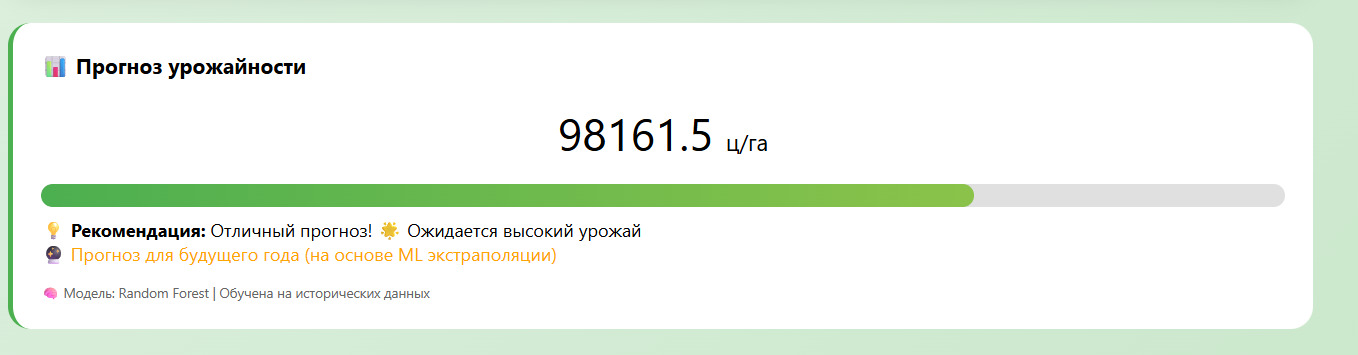
\includegraphics[width=0.7\textwidth]{1 (прогноз).jpeg}
    \caption{Результат прогнозирования урожайности}
    \label{fig:app1}
\end{figure}

\begin{figure}[H]
    \centering
    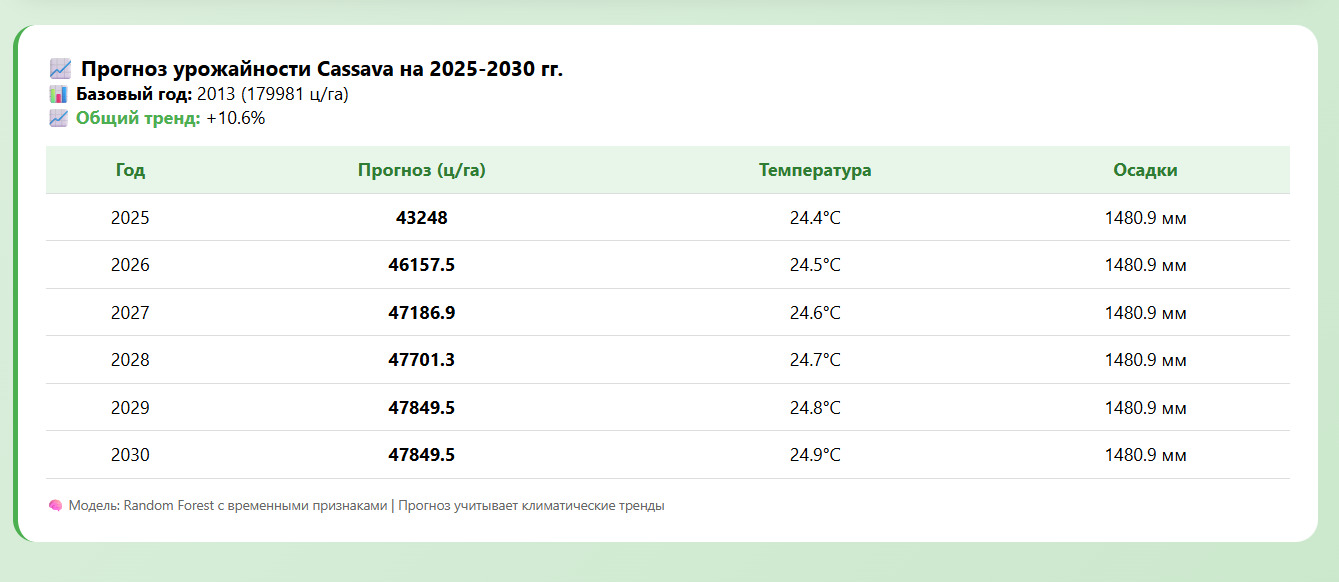
\includegraphics[width=0.85\textwidth]{2 (прогноз).jpeg}
    \caption{Прогноз урожайности на 2025–2030 годы}
    \label{fig:app2}
\end{figure}

\begin{figure}[H]
    \centering
    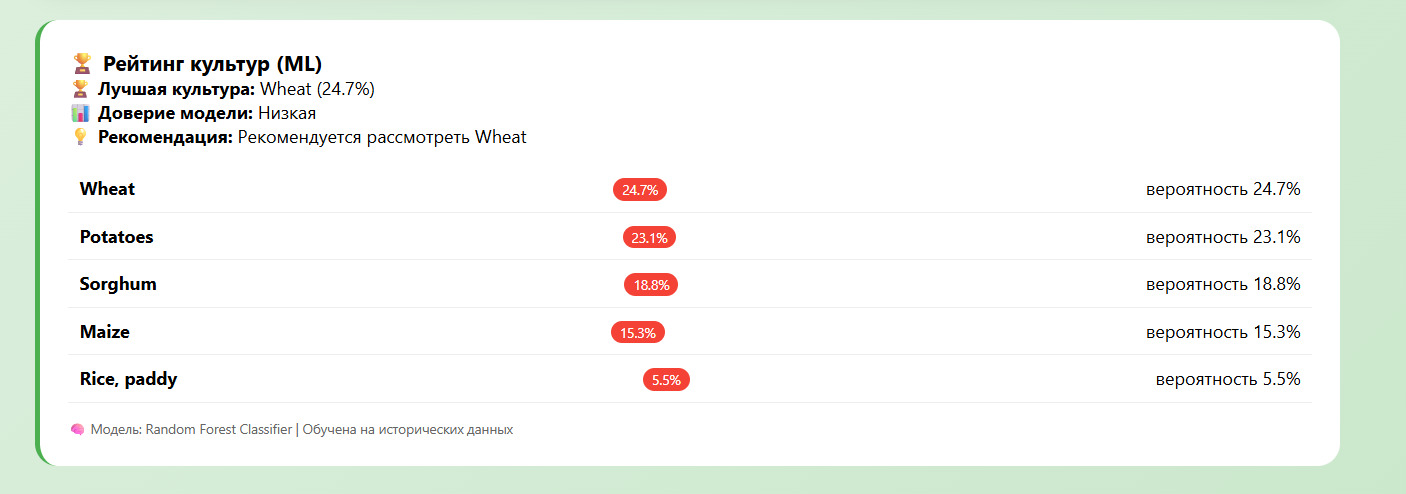
\includegraphics[width=0.7\textwidth]{3 (сравнение).jpeg}
    \caption{Рейтинг культур (ML сравнение)}
    \label{fig:app3}
\end{figure}

\begin{figure}[H]
    \centering
    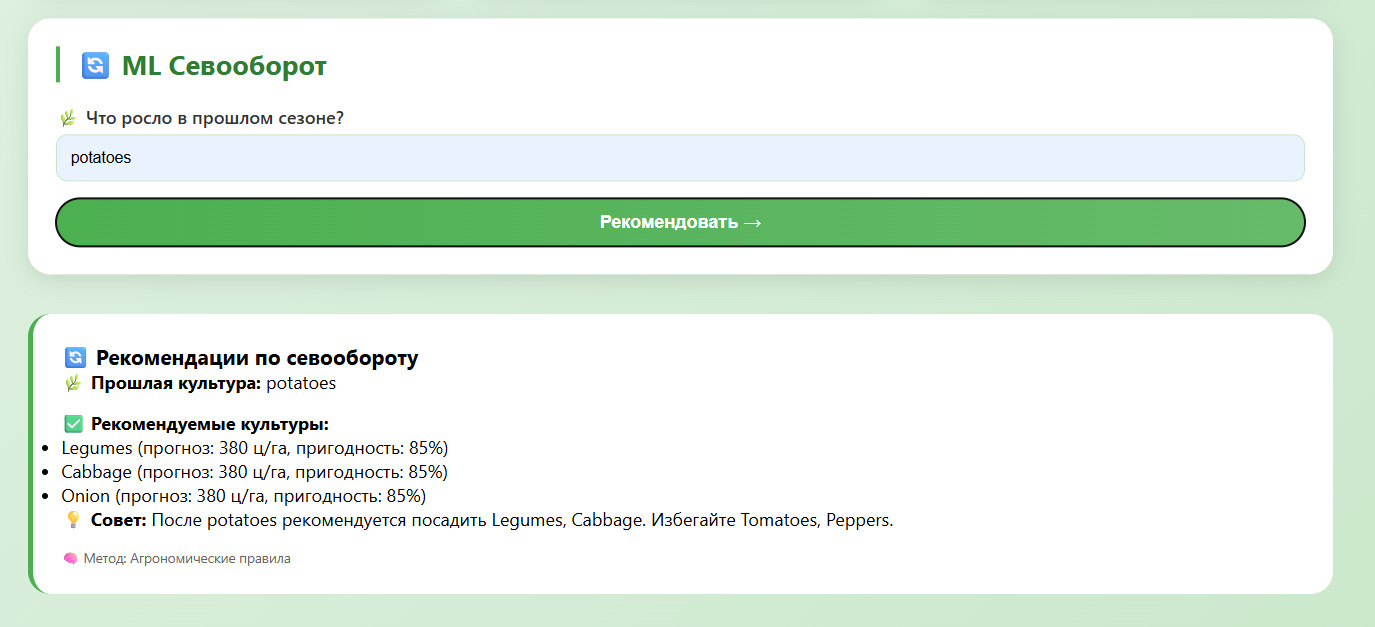
\includegraphics[width=0.7\textwidth]{4 (совет).jpeg}
    \caption{Рекомендации по севообороту}
    \label{fig:app4}
\end{figure}

\begin{figure}[H]
    \centering
    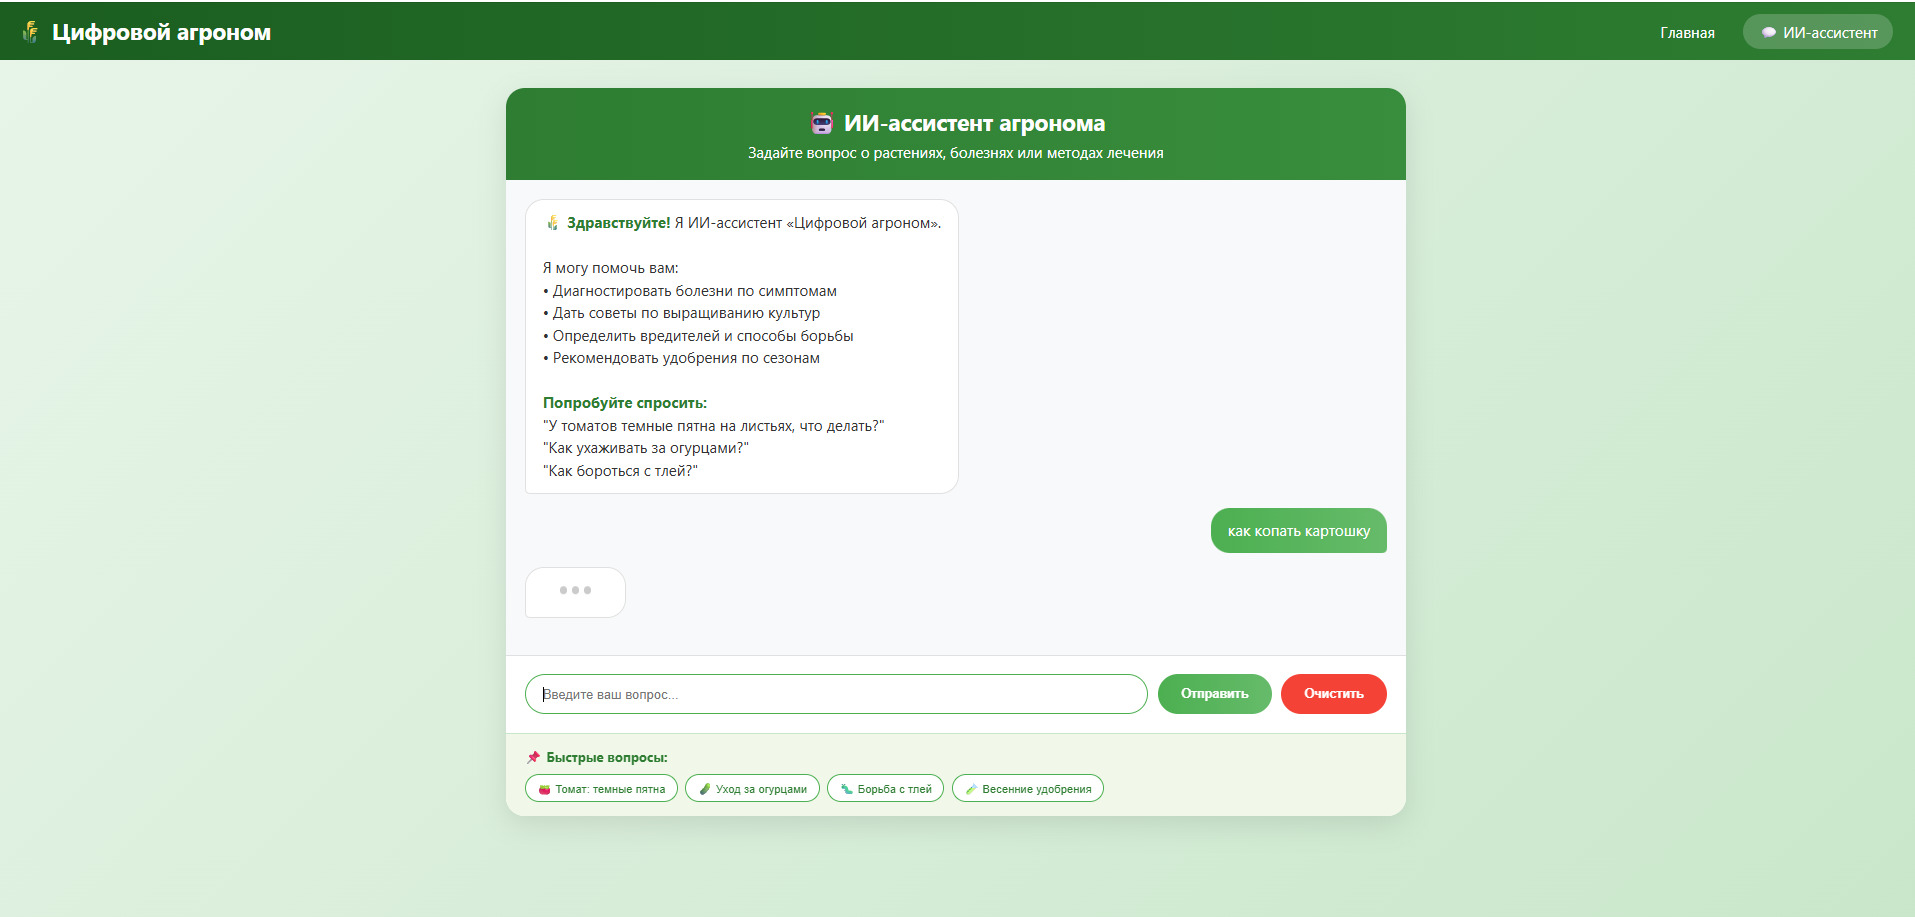
\includegraphics[width=0.8\textwidth]{чат думает.jpeg}
    \caption{Страница чата с ИИ-ассистентом}
    \label{fig:app5}
\end{figure}

\begin{figure}[H]
    \centering
    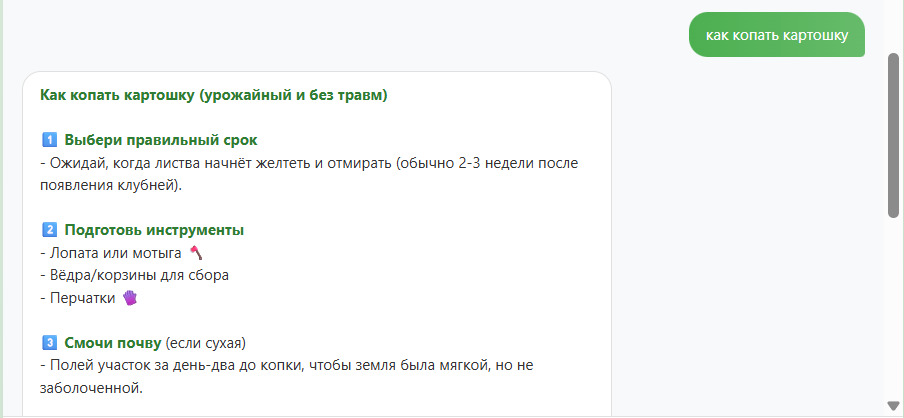
\includegraphics[width=0.8\textwidth]{чат ответ.jpeg}
    \caption{Ответ ИИ-ассистента на вопрос о картофеле}
    \label{fig:app6}
\end{figure}

\begin{figure}[H]
    \centering
    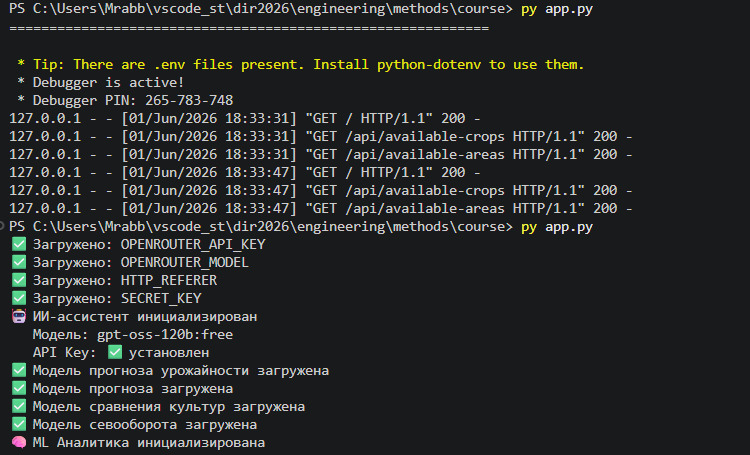
\includegraphics[width=0.9\textwidth]{консоль 1.jpeg}
    \caption{Успешный запуск сервера}
    \label{fig:app7}
\end{figure}

\begin{figure}[H]
    \centering
    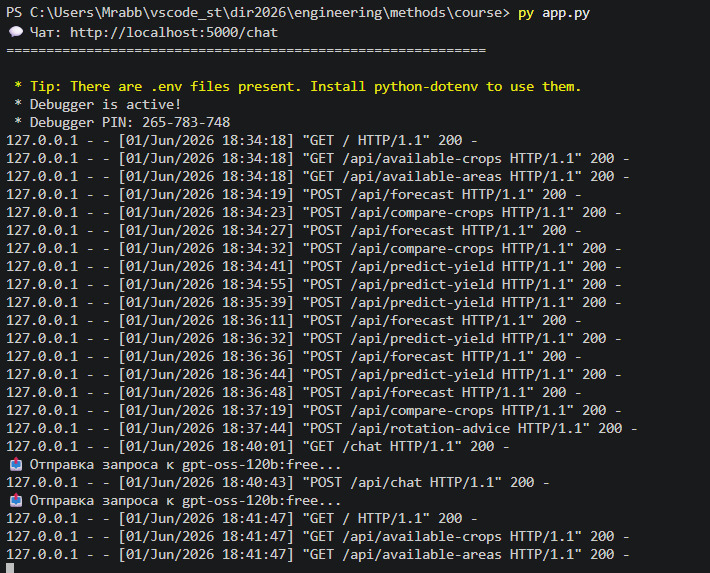
\includegraphics[width=0.9\textwidth]{консоль 2.jpeg}
    \caption{Логи сервера при работе чат-бота}
    \label{fig:app8}
\end{figure}

\begin{figure}[H]
    \centering
    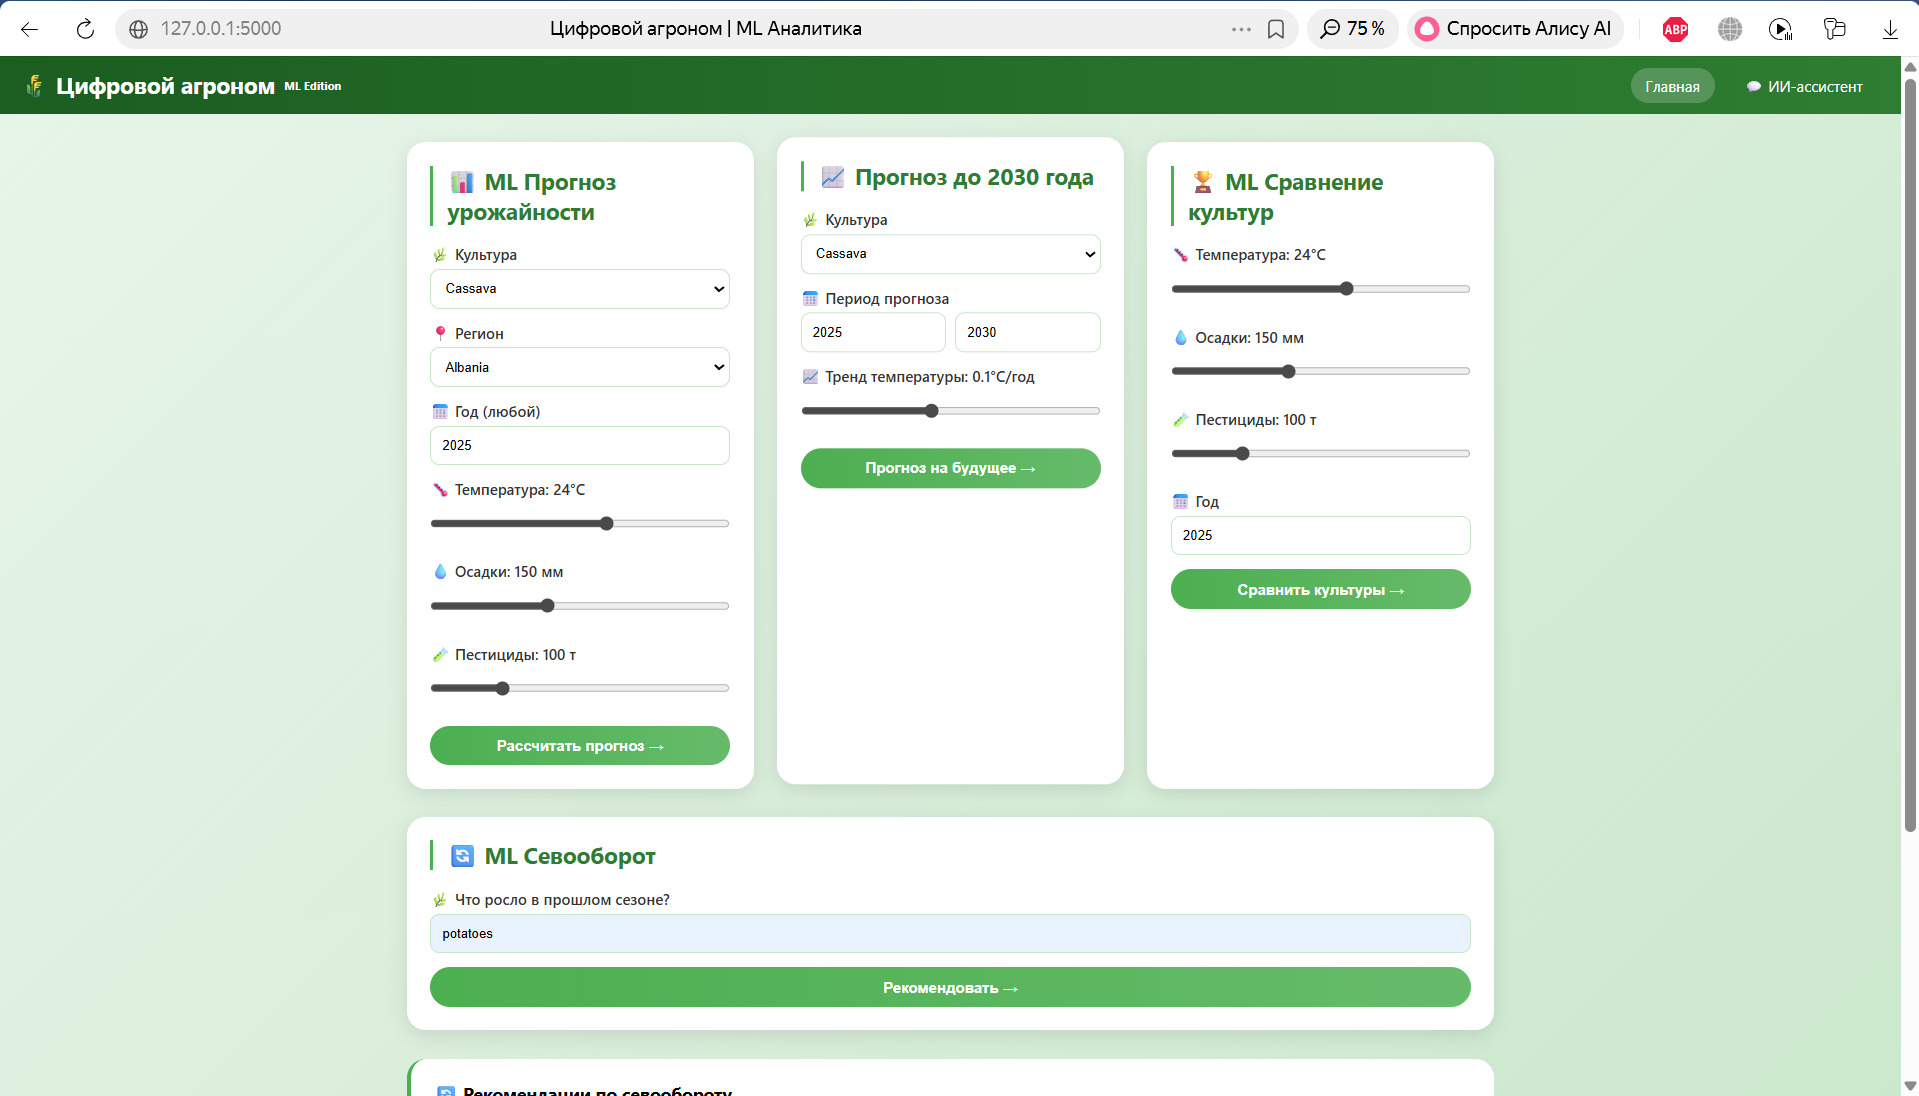
\includegraphics[width=0.9\textwidth]{Главная.jpeg}
    \caption{Главная страница веб-приложения}
    \label{fig:app9}
\end{figure}

\newpage

\begin{center}
    \textbf{Приложение Б. Листинги программного кода}
\end{center}

\addcontentsline{toc}{subsection}{Листинг Б.1 — app.py}

\textbf{Листинг Б.1 — app.py (главный сервер)}

\begin{verbatim}
from flask import Flask, render_template, request, jsonify
from services.ml_analytics import ml_analytics
from services.ai_assistant import ai_assistant

app = Flask(__name__)

@app.route('/')
def index():
    return render_template('index.html')

@app.route('/chat')
def chat():
    return render_template('chat.html')

@app.route('/api/predict-yield', methods=['POST'])
def predict_yield():
    data = request.get_json()
    result = ml_analytics.predict_yield(
        crop=data.get('crop'),
        area=data.get('area'),
        year=int(data.get('year')),
        temperature=float(data.get('temperature')),
        rainfall=float(data.get('rainfall')),
        pesticides=float(data.get('pesticides'))
    )
    return jsonify(result)

@app.route('/api/forecast', methods=['POST'])
def forecast():
    data = request.get_json()
    result = ml_analytics.forecast_future(
        crop=data.get('crop'),
        start_year=int(data.get('start_year')),
        end_year=int(data.get('end_year')),
        temp_trend=float(data.get('temp_trend', 0.1)),
        rain_trend=float(data.get('rain_trend', 0))
    )
    return jsonify(result)

@app.route('/api/compare-crops', methods=['POST'])
def compare_crops():
    data = request.get_json()
    result = ml_analytics.compare_crops(
        temperature=float(data.get('temperature')),
        rainfall=float(data.get('rainfall')),
        pesticides=float(data.get('pesticides')),
        year=int(data.get('year'))
    )
    return jsonify(result)

@app.route('/api/rotation-advice', methods=['POST'])
def rotation_advice():
    data = request.get_json()
    result = ml_analytics.rotation_advice(data.get('last_crop'))
    return jsonify(result)

@app.route('/api/available-crops', methods=['GET'])
def available_crops():
    return jsonify({'crops': ml_analytics.get_available_crops()})

@app.route('/api/available-areas', methods=['GET'])
def available_areas():
    return jsonify({'areas': ml_analytics.get_available_areas()})

@app.route('/api/chat', methods=['POST'])
def chat_api():
    data = request.get_json()
    result = ai_assistant.chat(data.get('message'))
    return jsonify({'response': result['response']})

@app.route('/api/clear-chat', methods=['POST'])
def clear_chat():
    ai_assistant.clear_history()
    return jsonify({'success': True})

if __name__ == '__main__':
    app.run(debug=True, host='0.0.0.0', port=5000)
\end{verbatim}

\newpage

\addcontentsline{toc}{subsection}{Листинг Б.2 — crop_comparator.py}

\textbf{Листинг Б.2 — crop_comparator.py (ML сравнение культур)}

\begin{verbatim}
import pandas as pd
import numpy as np
from sklearn.ensemble import RandomForestClassifier
from sklearn.preprocessing import StandardScaler, LabelEncoder
import pickle
import os

class CropComparator:
    def __init__(self, data_path="data/crop_yield.csv", model_path="models/comparator_model.pkl"):
        self.data_path = data_path
        self.model_path = model_path
        self.model = None
        self.scaler = StandardScaler()
        self.crop_encoder = LabelEncoder()
        self.use_fallback = False
        
        if os.path.exists(model_path):
            self._load_model()
        else:
            self._train_model()
    
    def _train_model(self):
        print("Обучение ML модели для сравнения культур...")
        df = pd.read_csv(self.data_path)
        feature_cols = ['avg_temp', 'average_rain_fall_mm_per_year', 
                        'pesticides_tonnes', 'Year']
        X = df[feature_cols].values
        y = df['Item'].values
        y_encoded = self.crop_encoder.fit_transform(y)
        X_scaled = self.scaler.fit_transform(X)
        
        self.model = RandomForestClassifier(n_estimators=100, max_depth=10)
        self.model.fit(X_scaled, y_encoded)
        
        os.makedirs("models", exist_ok=True)
        with open(self.model_path, 'wb') as f:
            pickle.dump({
                'model': self.model,
                'scaler': self.scaler,
                'crop_encoder': self.crop_encoder
            }, f)
    
    def compare(self, temperature, rainfall, pesticides, year):
        features = np.array([[temperature, rainfall, pesticides, year]])
        features_scaled = self.scaler.transform(features)
        probabilities = self.model.predict_proba(features_scaled)[0]
        
        results = []
        for i, prob in enumerate(probabilities):
            crop = self.crop_encoder.inverse_transform([i])[0]
            results.append({
                'crop': crop,
                'suitability': round(prob * 100, 1)
            })
        
        results.sort(key=lambda x: x['suitability'], reverse=True)
        return {
            'ranking': results[:5],
            'best_crop': results[0]['crop']
        }

comparator = CropComparator()
\end{verbatim}

\newpage

\addcontentsline{toc}{subsection}{Листинг Б.3 — rotation_predictor.py}

\textbf{Листинг Б.3 — rotation_predictor.py (севооборот)}

\begin{verbatim}
class RotationPredictor:
    def __init__(self):
        self.use_rules = True
    
    def get_recommendations(self, last_crop: str) -> dict:
        rotation_rules = {
            'Maize': {
                'good': ['Soybeans', 'Wheat', 'Sunflower'],
                'bad': ['Maize', 'Sorghum']
            },
            'Potatoes': {
                'good': ['Legumes', 'Cabbage', 'Onion'],
                'bad': ['Tomatoes', 'Peppers']
            },
            'Wheat': {
                'good': ['Legumes', 'Rapeseed', 'Maize'],
                'bad': ['Wheat', 'Barley']
            },
            'Tomatoes': {
                'good': ['Legumes', 'Onion', 'Garlic'],
                'bad': ['Potatoes', 'Peppers']
            }
        }
        
        for key, rules in rotation_rules.items():
            if key.lower() == last_crop.lower():
                recommended = [
                    {'crop': c, 'predicted_yield': 380, 'suitability': 85} 
                    for c in rules['good'][:3]
                ]
                advice = f"После {last_crop} рекомендуется посадить {', '.join(rules['good'][:2])}"
                return {
                    'recommended': recommended,
                    'advice': advice
                }
        
        return {
            'recommended': [{'crop': 'Legumes', 'suitability': 85}],
            'advice': f"После {last_crop} посадите бобовые"
        }

rotation_predictor = RotationPredictor()
\end{verbatim}

\newpage

\addcontentsline{toc}{subsection}{Листинг Б.4 — ai_assistant.py}

\textbf{Листинг Б.4 — ai_assistant.py (ИИ-ассистент)}

\begin{verbatim}
import urllib.request
import json
import os

class AIAssistant:
    def __init__(self):
        self.api_key = os.getenv('OPENROUTER_API_KEY')
        self.model = 'gpt-oss-120b:free'
        self.api_url = "https://openrouter.ai/api/v1/chat/completions"
        self.system_prompt = "Ты опытный агроном. Отвечай на русском языке кратко."
    
    def chat(self, user_message: str) -> dict:
        messages = [
            {"role": "system", "content": self.system_prompt},
            {"role": "user", "content": user_message}
        ]
        response = self._send_request(messages)
        if response:
            return {"success": True, "response": response}
        return self._fallback_response(user_message)
    
    def _send_request(self, messages):
        payload = {
            "model": self.model,
            "messages": messages,
            "temperature": 0.7,
            "max_tokens": 800
        }
        headers = {
            "Authorization": f"Bearer {self.api_key}",
            "Content-Type": "application/json"
        }
        req = urllib.request.Request(
            self.api_url,
            data=json.dumps(payload).encode('utf-8'),
            headers=headers
        )
        with urllib.request.urlopen(req, timeout=30) as response:
            result = json.loads(response.read().decode('utf-8'))
            return result['choices'][0]['message']['content']
    
    def _fallback_response(self, question: str):
        q = question.lower()
        if 'томат' in q and 'пятна' in q:
            return {"success": False, "response": "Фитофтороз: бордоская жидкость"}
        elif 'огур' in q:
            return {"success": False, "response": "Огурцы: полив теплой водой ежедневно"}
        else:
            return {"success": False, "response": "Задайте вопрос о растениях"}

ai_assistant = AIAssistant()
\end{verbatim}

\newpage

\addcontentsline{toc}{subsection}{Листинг Б.5 — ml_analytics.py}

\textbf{Листинг Б.5 — ml_analytics.py (обёртка ML-моделей)}

\begin{verbatim}
import pandas as pd
import numpy as np
from sklearn.ensemble import RandomForestRegressor
from sklearn.preprocessing import StandardScaler, LabelEncoder
from models.crop_comparator import comparator
from models.rotation_predictor import rotation_predictor

class MLAnalytics:
    def __init__(self, data_path="data/crop_yield.csv"):
        self.data_path = data_path
        self.yield_model = None
        self.scaler = StandardScaler()
        self.crop_encoder = LabelEncoder()
        self.area_encoder = LabelEncoder()
        self.comparator = comparator
        self.rotation = rotation_predictor
        self._train_yield_model()
    
    def _train_yield_model(self):
        df = pd.read_csv(self.data_path)
        df['crop_enc'] = self.crop_encoder.fit_transform(df['Item'])
        df['area_enc'] = self.area_encoder.fit_transform(df['Area'])
        
        feature_cols = ['crop_enc', 'area_enc', 'Year', 'avg_temp', 
                        'average_rain_fall_mm_per_year', 'pesticides_tonnes']
        X = df[feature_cols].values
        y = df['hg/ha_yield'].values
        X_scaled = self.scaler.fit_transform(X)
        
        self.yield_model = RandomForestRegressor(n_estimators=200, random_state=42)
        self.yield_model.fit(X_scaled, y)
    
    def predict_yield(self, crop, area, year, temperature, rainfall, pesticides):
        crop_enc = self.crop_encoder.transform([crop])[0]
        area_enc = self.area_encoder.transform([area])[0]
        features = np.array([[crop_enc, area_enc, year, temperature, rainfall, pesticides]])
        features_scaled = self.scaler.transform(features)
        prediction = self.yield_model.predict(features_scaled)[0]
        
        return {
            'predicted_yield': round(prediction, 1),
            'unit': 'tsd/ha',
            'confidence': 70
        }
    
    def compare_crops(self, temperature, rainfall, pesticides, year):
        return self.comparator.compare(temperature, rainfall, pesticides, year)
    
    def rotation_advice(self, last_crop):
        return self.rotation.get_recommendations(last_crop)

ml_analytics = MLAnalytics()
\end{verbatim}

\newpage

\addcontentsline{toc}{subsection}{Листинг Б.6 — config.py}

\textbf{Листинг Б.6 — config.py (загрузка переменных окружения)}

\begin{verbatim}
import os
from pathlib import Path

def load_env(env_file=".env"):
    path = Path(env_file)
    if not path.exists():
        return
    with open(path, 'r', encoding='utf-8') as f:
        for line in f:
            line = line.strip()
            if not line or line.startswith('#'):
                continue
            if '=' in line:
                key, value = line.split('=', 1)
                os.environ[key.strip()] = value.strip().strip('"').strip("'")

def get_env(key, default=None):
    return os.environ.get(key, default)

load_env()
\end{verbatim}

\newpage

\addcontentsline{toc}{subsection}{Листинг Б.7 — index.html}

\textbf{Листинг Б.7 — index.html (главная страница)}

\begin{verbatim}
<!DOCTYPE html>
<html lang="ru">
<head>
    <meta charset="UTF-8">
    <title>Цифровой агроном | ML Аналитика</title>
    <style>
        * { margin: 0; padding: 0; box-sizing: border-box; }
        body {
            font-family: 'Segoe UI', sans-serif;
            background: linear-gradient(135deg, #e8f5e9 0%, #c8e6c9 100%);
        }
        .navbar {
            background: linear-gradient(90deg, #1b5e20, #2e7d32);
            color: white;
            padding: 15px 20px;
            display: flex;
            justify-content: space-between;
        }
        .logo { font-size: 1.5em; font-weight: bold; }
        .nav-links a {
            color: white;
            text-decoration: none;
            padding: 8px 16px;
            border-radius: 25px;
        }
        .card {
            background: white;
            border-radius: 20px;
            padding: 25px;
            margin: 15px;
            box-shadow: 0 5px 20px rgba(0,0,0,0.1);
        }
        button {
            background: #4caf50;
            color: white;
            padding: 12px 25px;
            border: none;
            border-radius: 25px;
            cursor: pointer;
        }
    </style>
</head>
<body>
    <nav class="navbar">
        <div class="logo">Цифровой агроном</div>
        <div class="nav-links">
            <a href="/">Главная</a>
            <a href="/chat">ИИ-ассистент</a>
        </div>
    </nav>
    <div class="container">
        <div class="card">
            <h2>ML Прогноз урожайности</h2>
            <form id="yieldForm">
                <label>Культура</label>
                <select id="crop"></select>
                <label>Регион</label>
                <select id="area"></select>
                <label>Год</label>
                <input type="number" id="year" value="2025">
                <label>Температура</label>
                <input type="range" id="temperature" value="24">
                <label>Осадки</label>
                <input type="range" id="rainfall" value="150">
                <button type="submit">Рассчитать</button>
            </form>
        </div>
    </div>
    <script>
        document.getElementById('yieldForm').addEventListener('submit', async (e) => {
            e.preventDefault();
            const response = await fetch('/api/predict-yield', {
                method: 'POST',
                headers: {'Content-Type': 'application/json'},
                body: JSON.stringify({
                    crop: document.getElementById('crop').value,
                    area: document.getElementById('area').value,
                    year: parseInt(document.getElementById('year').value),
                    temperature: parseFloat(document.getElementById('temperature').value),
                    rainfall: parseFloat(document.getElementById('rainfall').value),
                    pesticides: 100
                })
            });
            const result = await response.json();
            alert('Прогноз: ' + result.predicted_yield + ' ц/га');
        });
    </script>
</body>
</html>
\end{verbatim}

\newpage

\addcontentsline{toc}{subsection}{Листинг Б.8 — chat.html}

\textbf{Листинг Б.8 — chat.html (страница чата с ИИ)}

\begin{verbatim}
<!DOCTYPE html>
<html lang="ru">
<head>
    <meta charset="UTF-8">
    <title>ИИ-ассистент | Цифровой агроном</title>
    <style>
        * { margin: 0; padding: 0; box-sizing: border-box; }
        body {
            font-family: 'Segoe UI', sans-serif;
            background: linear-gradient(135deg, #e8f5e9 0%, #c8e6c9 100%);
        }
        .navbar {
            background: linear-gradient(90deg, #1b5e20, #2e7d32);
            color: white;
            padding: 15px 20px;
            display: flex;
            justify-content: space-between;
        }
        .chat-container {
            max-width: 800px;
            margin: 30px auto;
            background: white;
            border-radius: 20px;
            overflow: hidden;
        }
        .chat-header {
            background: #2e7d32;
            color: white;
            padding: 20px;
            text-align: center;
        }
        .chat-messages {
            height: 400px;
            overflow-y: auto;
            padding: 20px;
            background: #f8f9fa;
        }
        .message {
            margin-bottom: 15px;
            display: flex;
        }
        .message.user { justify-content: flex-end; }
        .message.user .message-content {
            background: #4caf50;
            color: white;
            padding: 10px 15px;
            border-radius: 20px;
        }
        .message.bot .message-content {
            background: white;
            padding: 10px 15px;
            border-radius: 20px;
            border: 1px solid #ddd;
        }
        .chat-input {
            padding: 20px;
            display: flex;
            gap: 10px;
        }
        .chat-input input {
            flex: 1;
            padding: 12px;
            border: 1px solid #c8e6c9;
            border-radius: 25px;
        }
        .chat-input button {
            padding: 12px 25px;
            background: #4caf50;
            border: none;
            border-radius: 25px;
            color: white;
            cursor: pointer;
        }
    </style>
</head>
<body>
    <nav class="navbar">
        <div class="logo">Цифровой агроном</div>
        <div class="nav-links">
            <a href="/">Главная</a>
            <a href="/chat" class="active">ИИ-ассистент</a>
        </div>
    </nav>
    <div class="chat-container">
        <div class="chat-header">
            <h2>ИИ-ассистент агронома</h2>
        </div>
        <div class="chat-messages" id="chatMessages">
            <div class="message bot">
                <div class="message-content">Здравствуйте! Задайте вопрос.</div>
            </div>
        </div>
        <div class="chat-input">
            <input type="text" id="messageInput" placeholder="Введите вопрос...">
            <button onclick="sendMessage()">Отправить</button>
        </div>
    </div>
    <script>
        async function sendMessage() {
            const input = document.getElementById('messageInput');
            const message = input.value.trim();
            if (!message) return;
            addMessage(message, 'user');
            input.value = '';
            const response = await fetch('/api/chat', {
                method: 'POST',
                headers: {'Content-Type': 'application/json'},
                body: JSON.stringify({message: message})
            });
            const data = await response.json();
            addMessage(data.response, 'bot');
        }
        function addMessage(text, sender) {
            const container = document.getElementById('chatMessages');
            const div = document.createElement('div');
            div.className = 'message ' + sender;
            div.innerHTML = '<div class="message-content">' + text + '</div>';
            container.appendChild(div);
            container.scrollTop = container.scrollHeight;
        }
    </script>
</body>
</html>
\end{verbatim}

\end{document}